\chapter{Methods | how to estimate luminosity class from color} \label{chap:METHODS}
% ========================

In this section, we present how we go from the original Michigan Spectral Catalogs to estimating probabilities of luminosity class for a star with a known spectral type and unknown luminosity class.

\section{``Cleaning'' the Michigan Spectral Catalog and cross-matching with 2MASS/WISE} \label{sec:clean_michigan}

We remove from the Michigan catalogs all targets with peculiar and/or mixed spectral types and luminosity classes (e.g. ``M2/3III'', ``G2e+K0V'', etc.).  The  number of targets in each Michigan Catalog with both a single spectral type and luminosity class assignment are typically $>$50\% and are listed in Table 1, with a total of $\sim$87,000 stars. We plot in Figure 1 the distribution of spectral types as a function of luminosity class of the ``cleaned'' sample from the Michigan Spectral Catalogs.  These histograms include the Michigan Spectral Atlas stars that do not have good positional cross-matches and photometry from 2MASS and WISE as described in ${\S}$2.2.

\begin{figure}[t]
    \begin{center}
        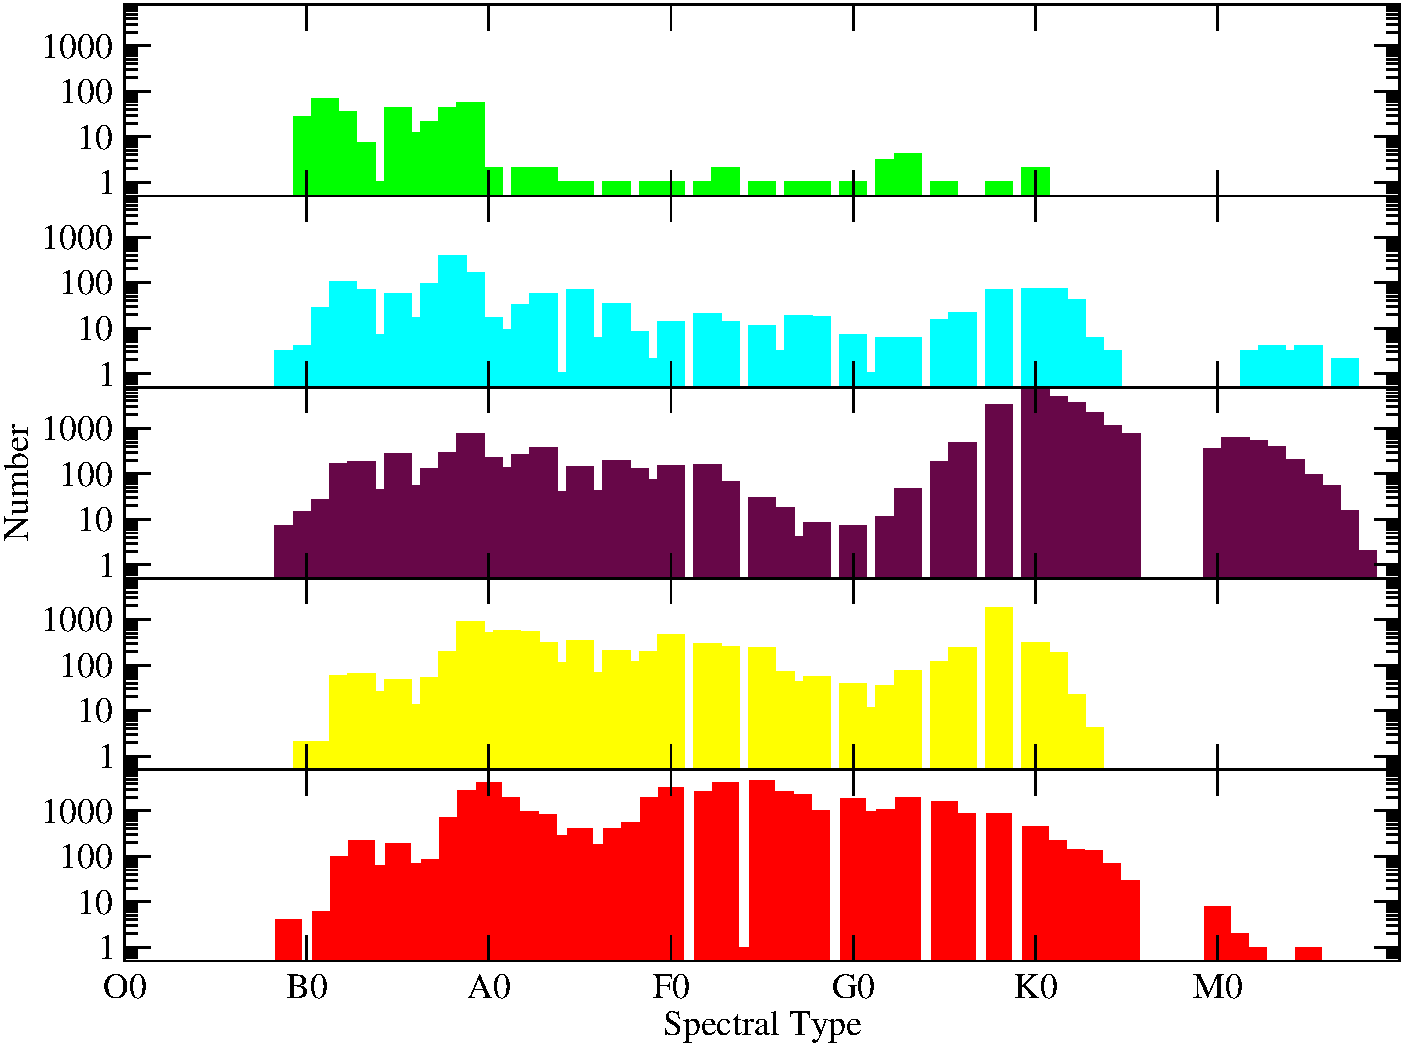
\includegraphics[width=1.0\textwidth]{Figures/populations/hist-spt-count.pdf}
    \end{center}
\caption{The distribution of the Michigan Spectral Catalogs as a function of spectral type on the horizontal axis, after the removal of peculiar and/or mixed spectral types.  The different colors correspond to the different luminosity classes.  From bottom to top: V (red), IV (yellow), III (purple), II (cyan) and I (green).  The gaps in the histograms at particular spectral types (e.g. F1, K7-K9) indicate that this spectral type was not used for typing in the Michigan Spectral Catalogs.}
\end{figure}

\section{Color as a probability density function}
% a lot of the text in 3.2 should go to figure 2/3 (median plot), fitting t-dist
\label{subsec:quant_color}

\begin{figure}
    \centering
    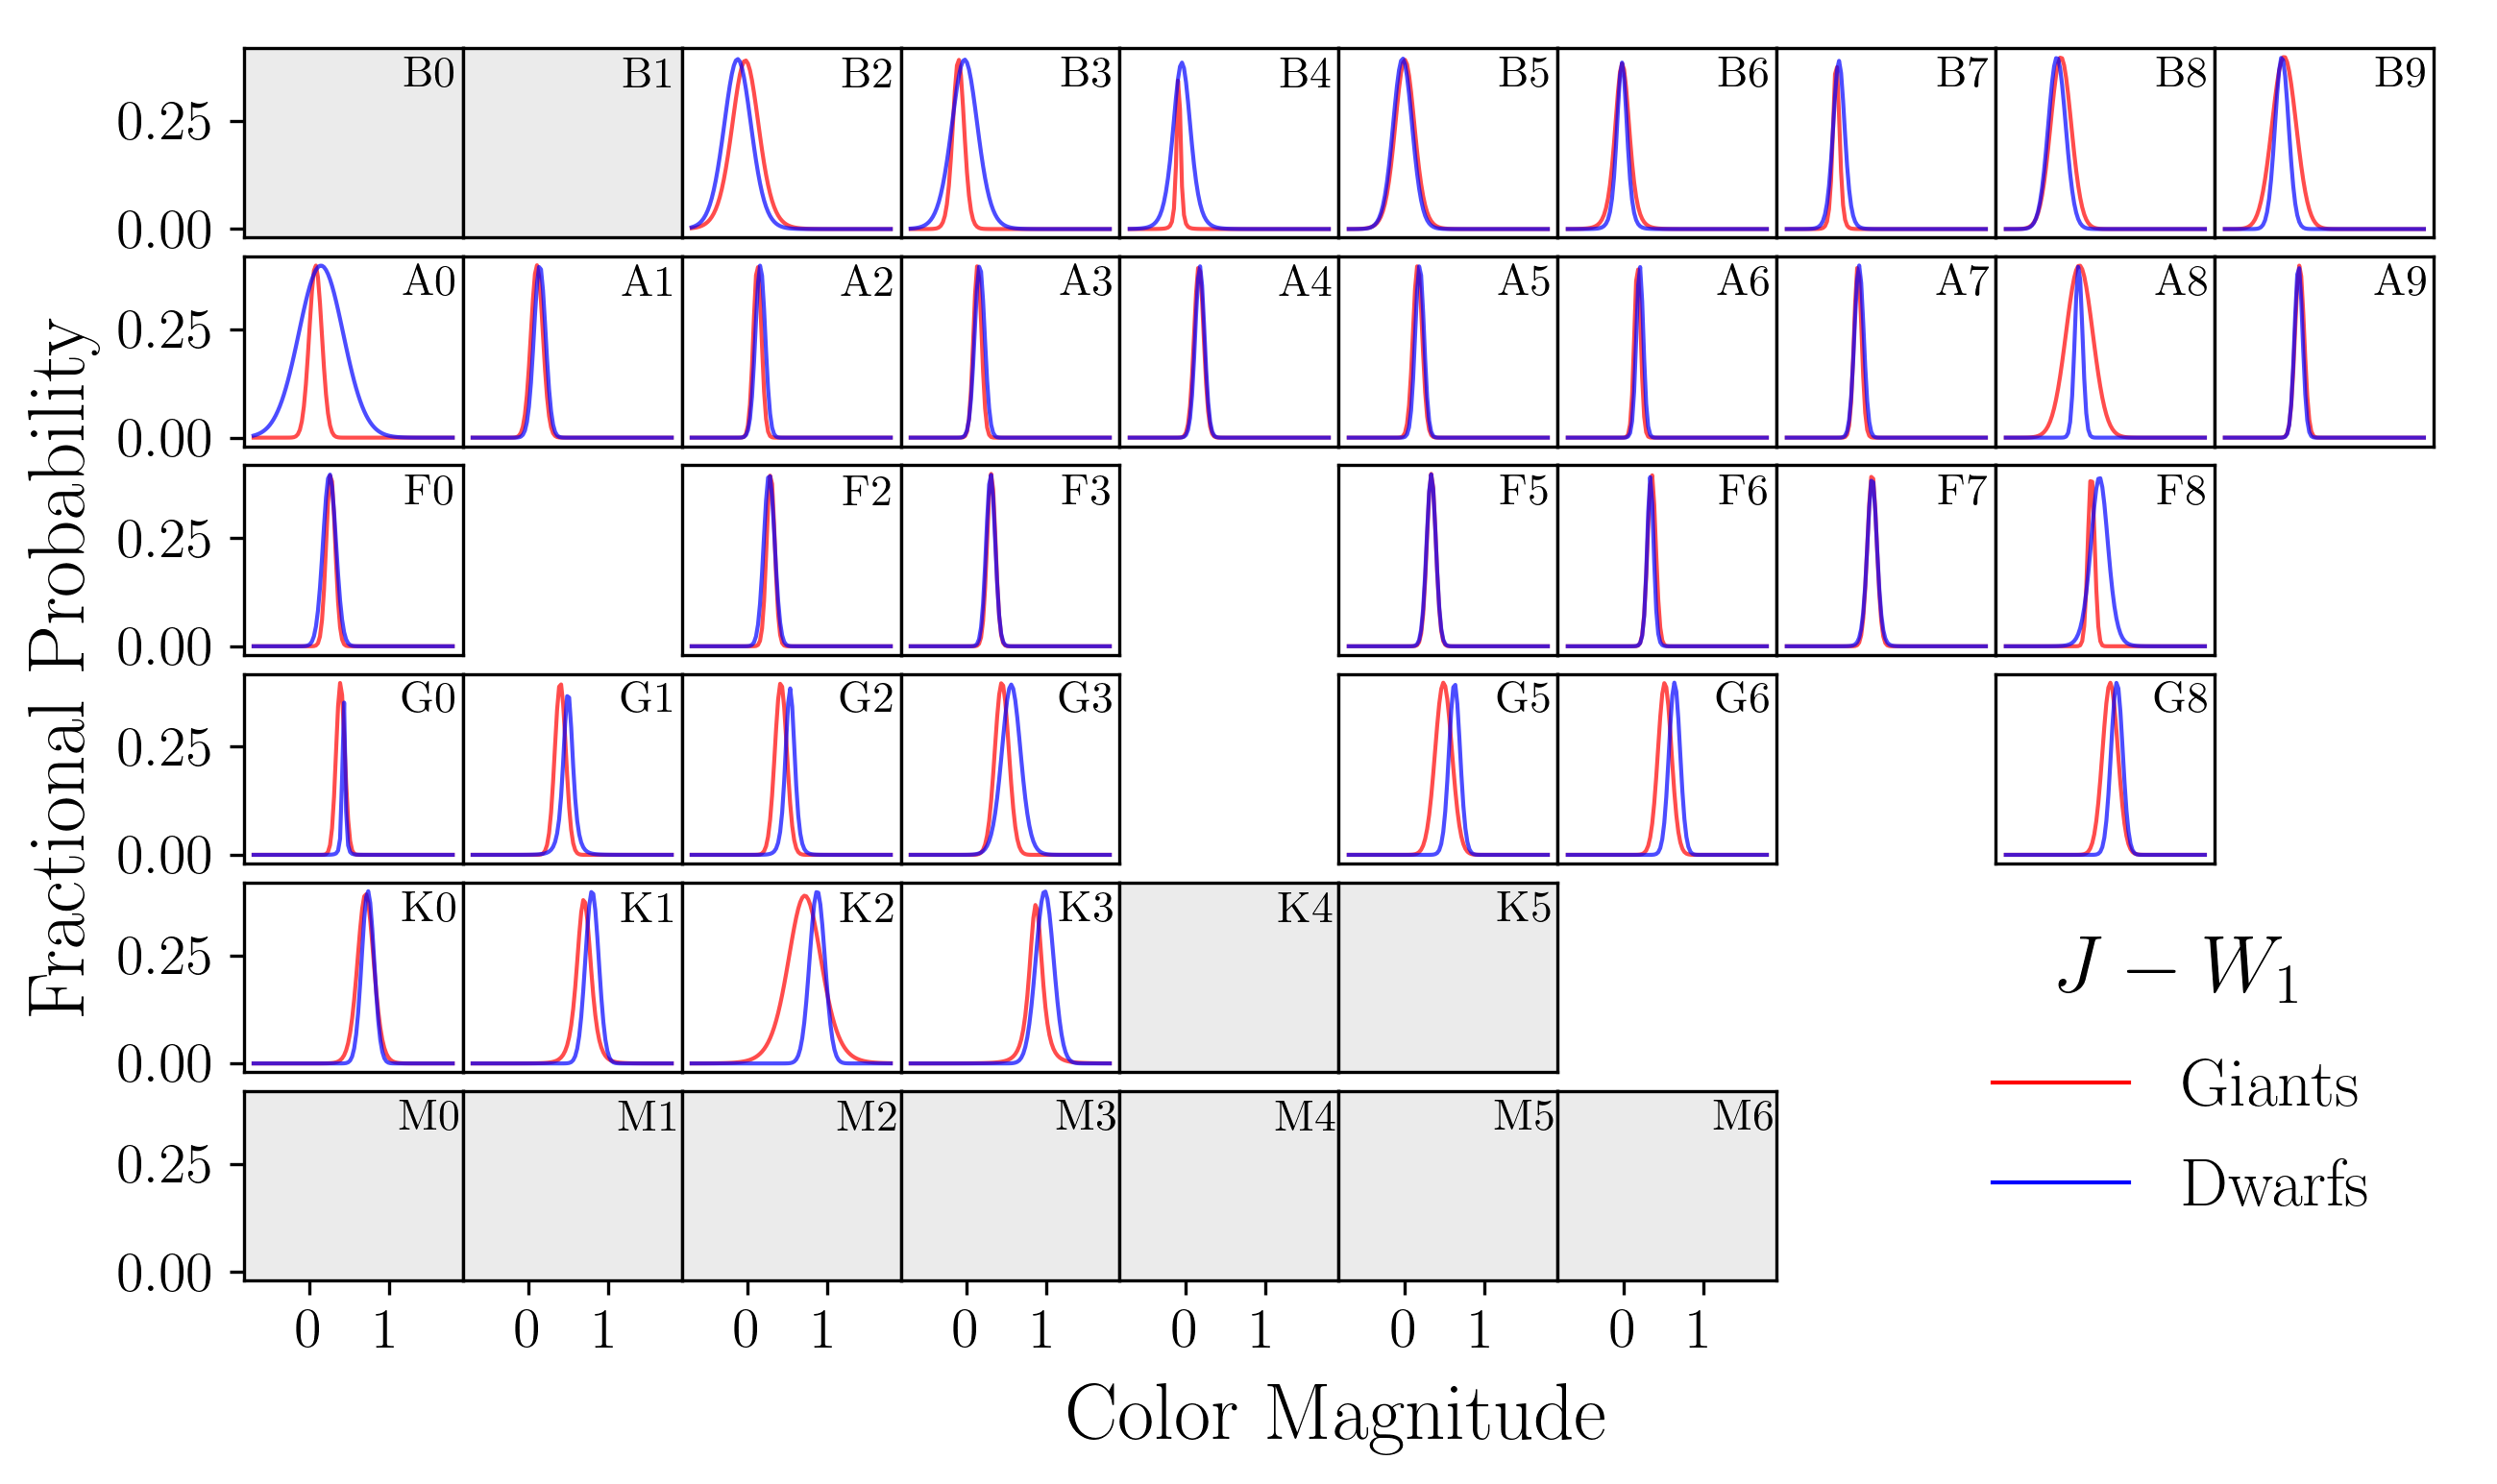
\includegraphics[width=1.0\textwidth,clip=true]{Figures/periodic/periodic-t-pdf_J_W1.png}
    \caption{Caption}
    \label{fig:periodic-pdf-jw1}
\end{figure}

\begin{figure}
    \centering
    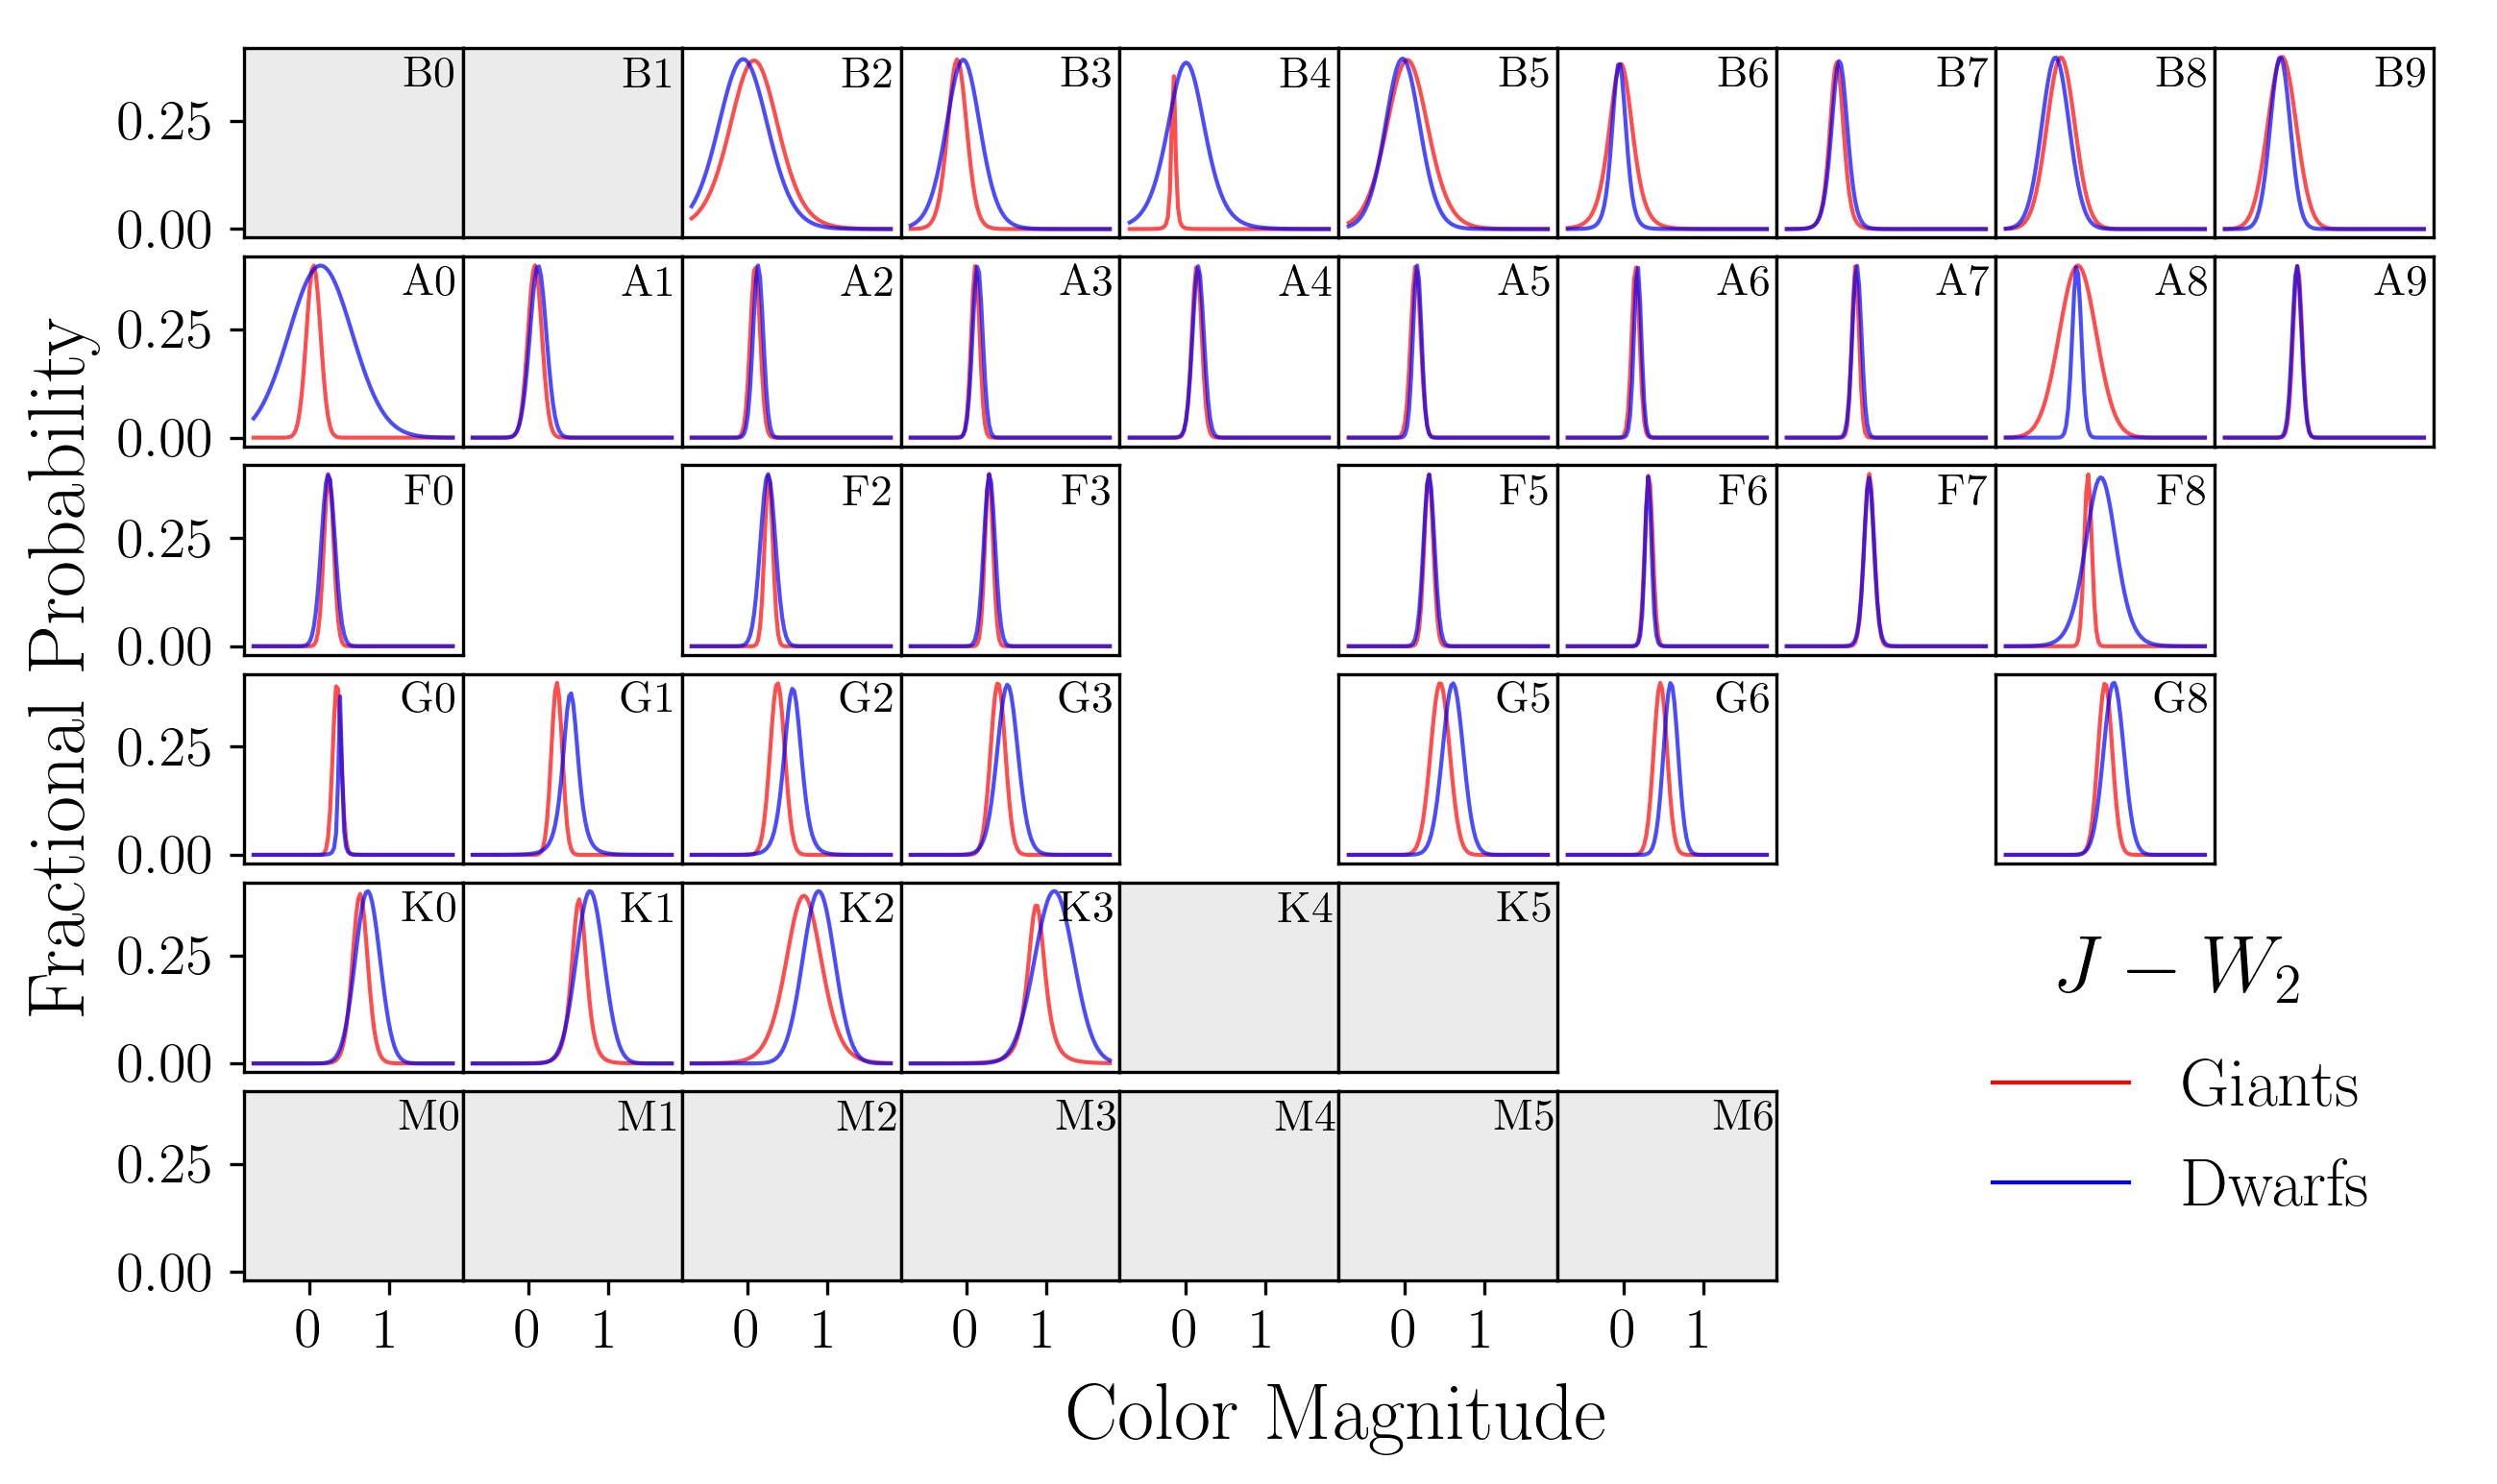
\includegraphics[width=1.0\textwidth,clip=true]{Figures/periodic/periodic-t-pdf_J_W2.png}
    \caption{Same as Figure \ref{fig:periodic-pdf-jw1}, but for \jwtwo.}
    \label{fig:periodic-pdf-jw2}
\end{figure}


From the photometry in ${\S}$2.2, for all stars that match a single spectral type and luminosity class, have good photometry measurements, and have a good positional cross-match between 2MASS and WISE, we calculate the median and robust standard deviation of stellar colors $J-H$, $J-K_s$, $H-K_s$, $J-W1$, $J-W2$, $J-W3$, $J-W4$, $H-W1$, $H-W2$, $H-W3$, $H-W4$, $K_s-W1$, $K_s-W2$, $K_s-W3$, $K_s-W4$, $W1-W2$, $W1-W3$, $W1-W4$, $W2-W3$, $W2-W4$, and $W3-W4$.  When only three stars are in a given spectral type and luminosity class bin for a given color, we compute the standard deviation rather than the robust standard deviation.  When only two stars are in a given spectral type and luminosity class bin for a given color, we compute the range rather than the robust standard deviation.  When only one star has a given spectral type and luminosity class, we do not compute a distribution range.  When zero stars are in a given spectral type and luminosity class, we do not compute a distribution median.  The colors and standard deviations of the Michigan Spectral Catalogs are listed as a function of spectral type and luminosity class in Tables 2-21, and plotted in Figures 2-4.


\begin{figure*}[t]
\centering
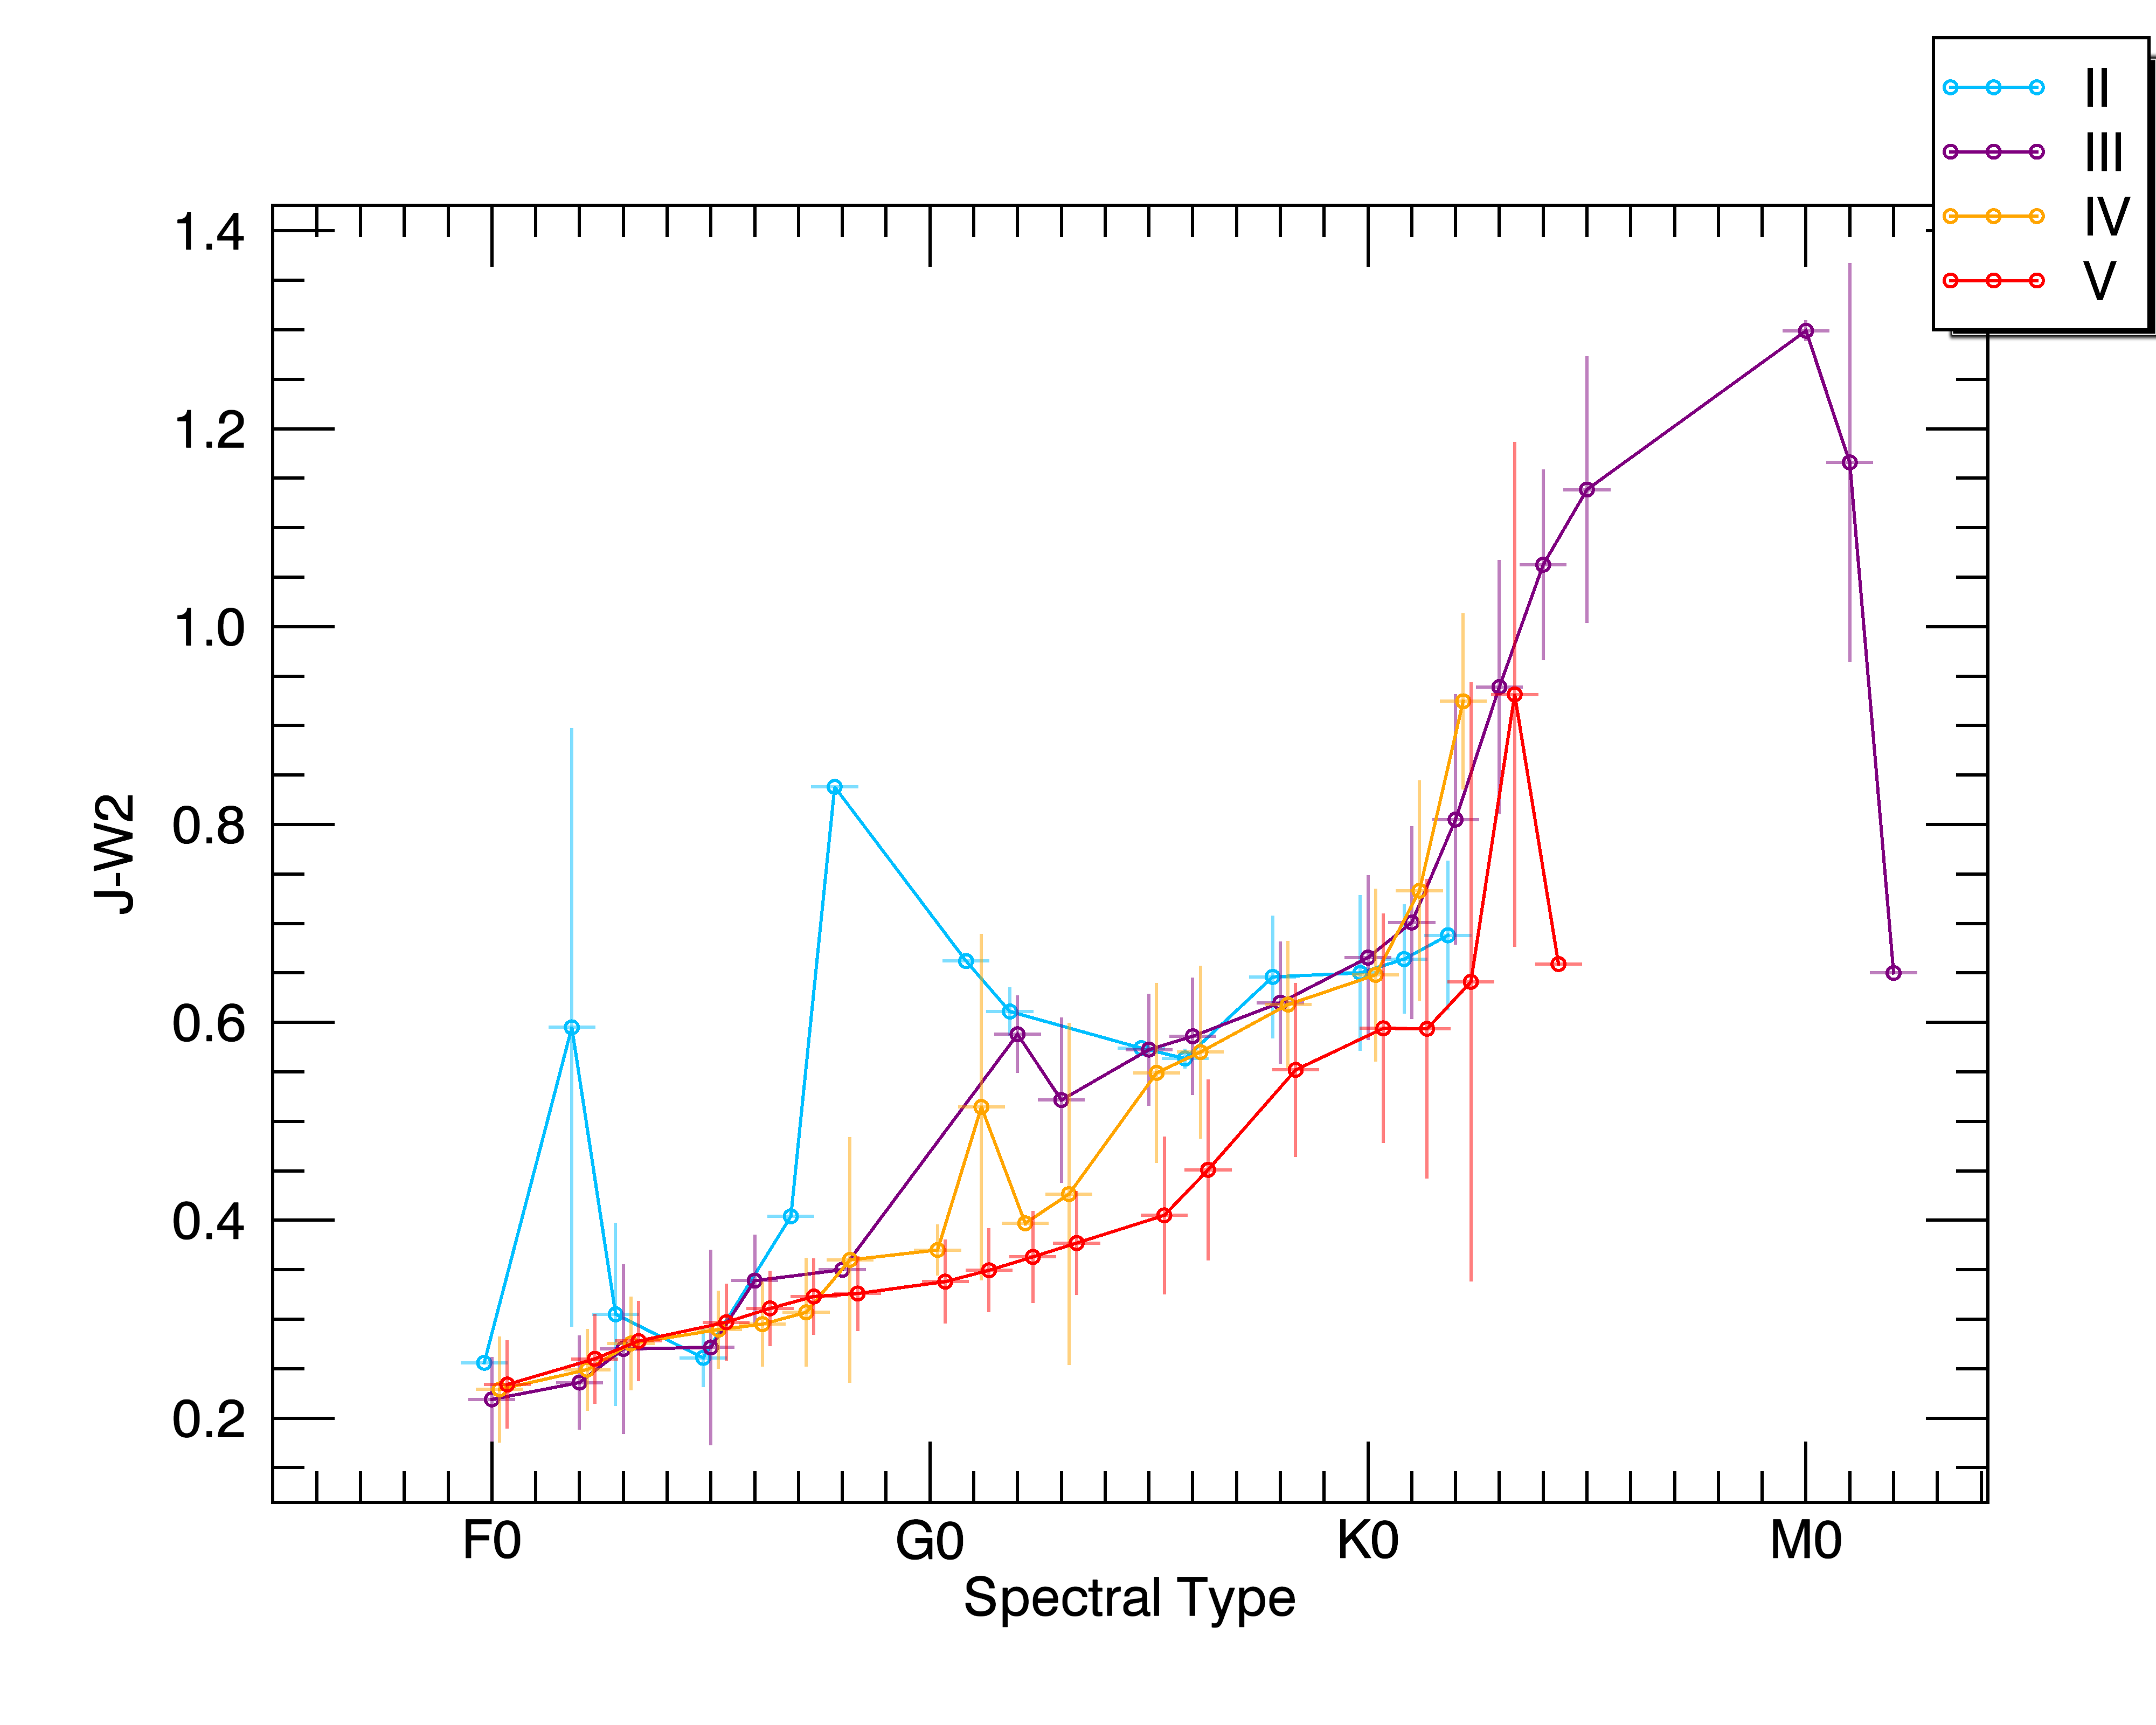
\includegraphics[width=1.0\textwidth,clip=true]{Figures/subtype_bar/SPT_J-W2.png}
 
\caption{The color of stars in the Michigan Spectral Catalogs as a function of spectral type on the horizontal axis, and \jwtwo on the vertical axis, after the removal of peculiar and/or mixed spectral types (see ${\S}$3.1). The different colors correspond to the different luminosity classes -- V (red), IV (yellow), III (purple), II (cyan) and I (green).  The vertical error bars generally correspond to the robust standard deviation of the \jwtwo color of stars within a given spectral type and luminosity class, unless there are only three or fewer stars, in which the error bars represent a standard deviation or range. (see ${\S}$3.2).}
\end{figure*}

\begin{figure*}[t]
%\ContinuedFloat
\centering  
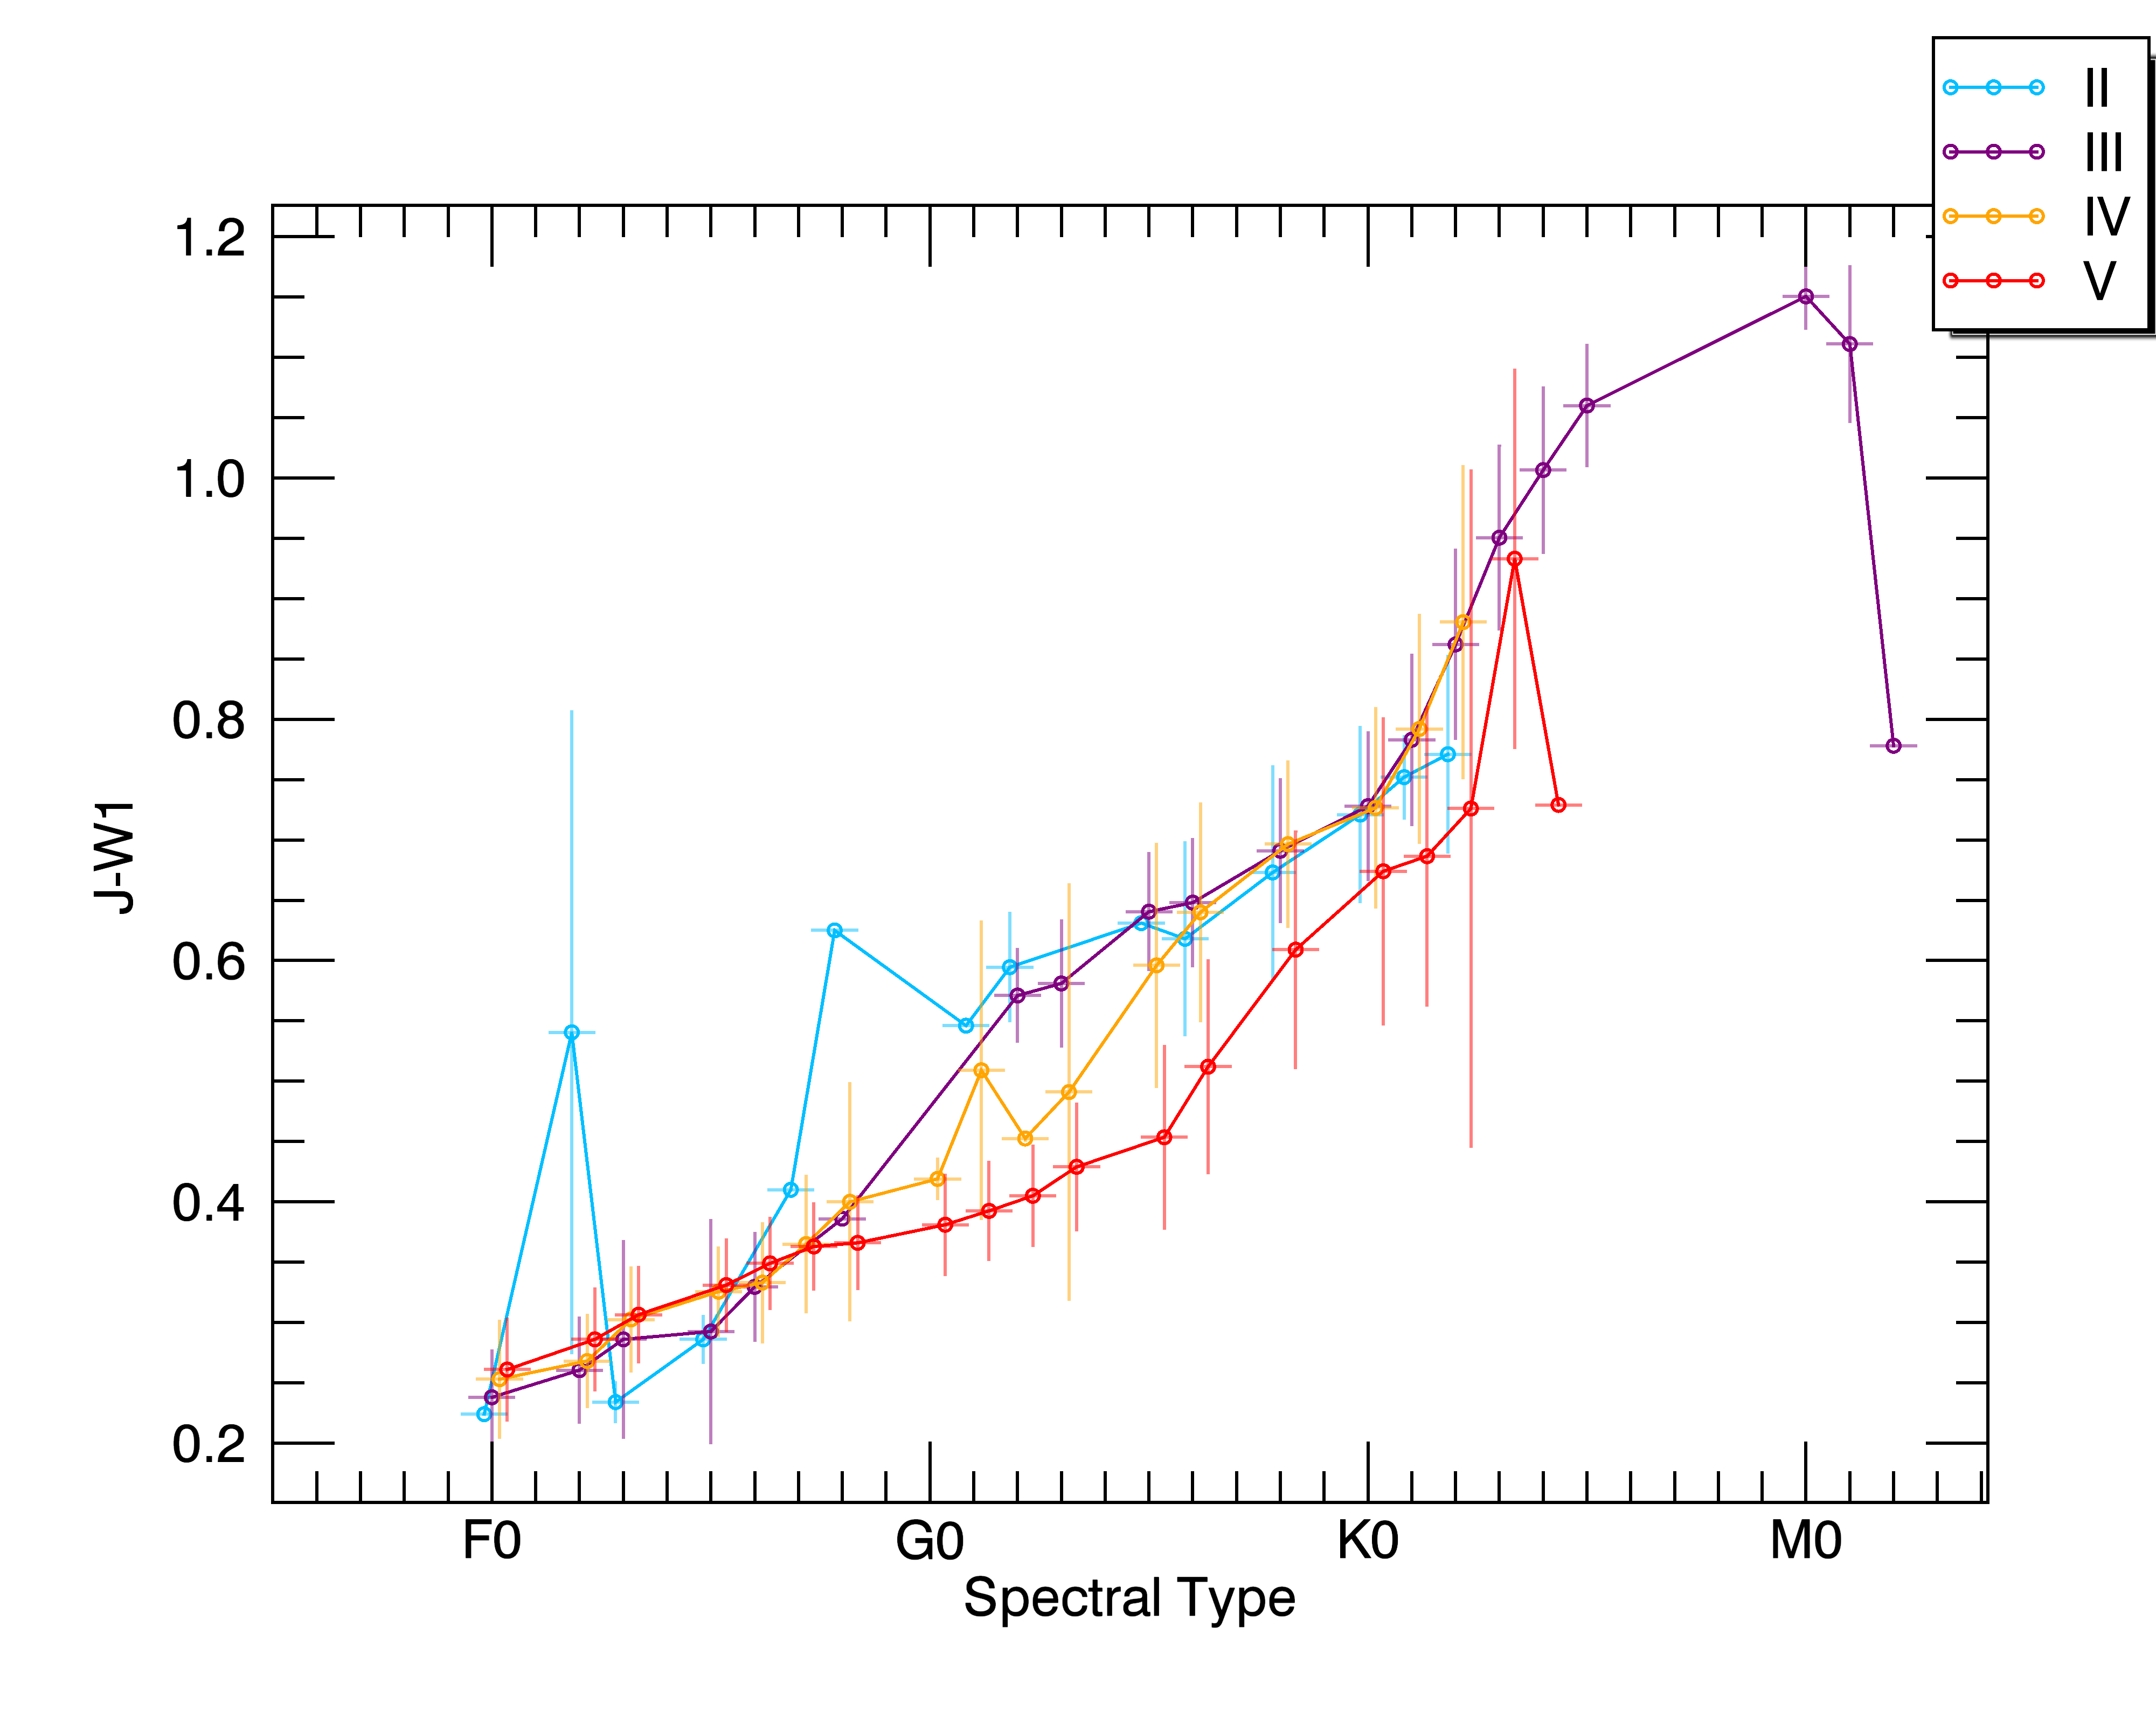
\includegraphics[width=1.0\textwidth,clip=true]{Figures/subtype_bar/SPT_J-W1.png}
\caption{The same as Figure 2, except for $J-W1$}
\end{figure*}

\section{How to infer luminosity class}

We search Tables 2-22 to identify colors where the luminosity class median colors differ substantially for a given contiguous range of spectral types.  We quantify 'substantially' when the difference in luminosity class median exceeds the standard deviation for the main sequence luminosity class $V$.  







